\documentclass[10pt,twoside,slovak,a4paper]{article}

\usepackage[slovak]{babel}
\usepackage[IL2]{fontenc}
\usepackage[utf8]{inputenc}
\usepackage{graphicx}
\usepackage{url}
\usepackage{hyperref}

\usepackage{cite}


\pagestyle{headings}

\title{Holistický prístup k tvorbe serióznych hier\thanks{Semestrálny projekt v predmete Metódy inžinierskej práce, ak. rok 2022/2023, vedenie: Zuzana Špitálová}} 

\author{Lukáš Michalčák\\[2pt]
{\small Slovenská technická univerzita v Bratislave}\\
{\small Fakulta informatiky a informačných technológií}\\
{\small \texttt{xmichalcak@stuba.sk}}
}

\date{\small 6. november 2022} 

\begin{document}

\maketitle

\begin{abstract}
Seriózne hry sú v akademickej či profesijnej sfére známe ako nástroje k odovzdávaniu vedomostí. Sú nazývané \emph{hrami}, pretože sú podobné bežným komerčným hrám v tom, že obsahujú aj element zábavy. Takto má teoreticky seriózna hra fungovať. V praxi to však vyzerá tak, že vo väčšine prípadov nastáva prevaha vzdelávacieho alebo zábavného elementu, čo je veľmi kontraproduktívne voči úmyslu hry. Z logického hľadiska by odpoveďou na tento problém bol vývoj hry, ktorá má oba elementy vyvážené. Preto je dôležitý vývin takej koncepcie herného dizajnu, ktorá by toto zabezpečovala.
\end{abstract}



\section{Úvod}

\paragraph{Historické súvislosti - história serióznych hier.} Seriózne hry ako vedecký odbor je veľmi mladý. Všeobecne existuje konsenzus, že jeho otcom je Clark C Abt, ktorý tento pojem vymyslel v 1970 a popularizátorom Ben Saywer od roku 2002. \cite{wilkinson2016brief} Avšak hlavný koncept za týmto pojmom - \emph{hra, ktorej primárny účel nie je zábava} \cite{alvarez2011introduction} - je možné vystopovať do dávnej minulosti, už do čias Platóna, ktorý sa vo svojich úvahách zaoberal myšlienkou divadelných hier, ktoré by slúžili na účel poučenia a vzdelávania a naozaj, keď sa pozrieme na mnohé divadelné hry histórie, ako napríklad od Williama Shakesphearea, môžeme aj v jeho komédiách nájsť mnoho poučného. Preto možno povedať, že táto myšlienka sprevádza ľudstvo v určitej podobe naprieč históriou.

\vspace{\baselineskip}

No napriek tomu, že táto myšlienka má korene už v dávnej minulosti a dnes sa jej rozvoju venuje celý vedný odbor, stále tvorcovia serióznych hier zápasia s jedným závažným problémom. Hoci je celkom samozrejmé, že optimálna seriózna hra by mala byť navrhnutá a implementovaná tak, aby v rovnakej miere prinášala zábavu i ponaučenie a aby tieto 2 aspekty navzájom prirodzene koexistovali a boli zdanlivo nerozlíšiteľné, pri aplikácii do reality sa zväčša veľmi nedarí toto naplniť. Výsledkom sú hry, ktoré sú príliš zamerané na zdieľanie kvanta informácií alebo, naopak, priorizujú zábavu a prinášajú málo vzdelania. Tento problém a jeho možné riešenie budú náplňou mojej práce.

O tom, na čom seriózne hry stavajú, sa budem venovať v časti \ref{ciel}.
Analýza vedeckých faktov na riešenie daného problému bude v časti \ref{jadro} .
Riešenie problému, inšpirované štúdiou \cite{natucci2021experience} a mnou modifikované v časti \ref{riesenie} .
Zhrnutie semestrálnej práce bude v časti \ref{zaver} .

\section{Z čoho pozostávajú seriózne hry} \label{ciel}
Základná myšlienka a podstata serióznych hier je samozrejmá z predostretej definície. Hlavnou otázkou teda je toto: Akými prostriedkami je toto možné dosiahnuť?
No, zdá sa že ju nie je jednoduché zodpovedať. Interpretácie toho, na aké koncepty by sa mala seriózna hra odvolávať sa líšia podľa zdroja, pretože neexistuje jednoznačný a všeobecne akceptovaný model. Preto som sa rozhodol vytvoriť model, ktorý by vyhovoval myšlienkovým modelom z čo najviac z tých zdrojov, ktoré sú uvedené na konci práce. Vyzeralo by to asi takto:

\begin{figure}[h]
\centering
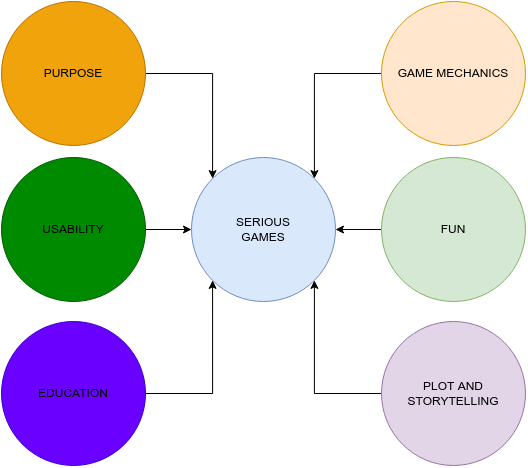
\includegraphics[width = 0.5\textwidth]{serious_games.png}
\caption{Zovšeobecnený model vlastností serióznych hier}
\label{fig:model}
\end{figure}

Z obrázku \ref{fig:model} sa dajú jasne rozpoznať kľúčové komponenty efektívnej serióznej hry. Tieto pojmy a ich súvislosti vysvetlím:
\paragraph{Cieľ.} Ten je celkom jasný, už som ho spomenul. Cieľom je vzdelávanie v nejakej oblasti a často aj nejaká sociálna či filozofická výzva spojená s tou témou, pričom prostriedkami tohto cieľa sú rozličné herné elementy. Problémom je však to, že v praxi je tento cieľ zatiaľ neefektívny, pretože zvykne byť len dočasný. Ukazuje sa totiž, že efekt je vo väčšine prípadov len dočasný, bez vyhliadok. Subjekty rôznych experimentov a štúdií preukázali, že seriózne hry môžu často byť neefektívne z dlhodobého hľadiska \cite{lewis2007analysis}. Ich problémom je teda aj udržateľnosť dosiahnutých výsledkov.
\paragraph{Udržateľnosť a etika.} Udržateľnosť je veľmi široký pojem a možno ho vnímať v rozličných kontextoch, udržateľnosť vo sfére ekológie v súvislosti s narábaním s prírodnými zdrojmi a životným prostredím, udržateľnosť fyzickej kondície ako súčasť zdravého životného štýlu, udržateľnosť softvéru po jeho vydaní, udržateľnosť pozornosti a výkonu,... Najmä posledné 2 úzko súvisia s problematikou serióznych hier. Častokrát sa developeri serióznych hier starajú o funkčnosť svojej hry len do dňa vydania hry, možno v minimálnej miere updatujú svoj softvér, ale všeobecne sa dá povedať, že neexistuje veľká iniciatíva o udržiavanie týchto hier, najmä ak nie sú veľmi náročné s hľadiska programovania a objemu zdrojového kódu. No chyby nastávajú aj v takýchto menších projektoch a treba na to brať ohľad.

Takisto má mnoho serióznych hier problém s dlhodobými a pretrvávajúcimi výsledkami , čo sa týka ich vzdelávacieho zámeru. Snažia sa totiž o tzv. vynútenú udržateľnosť, ktorá sa prejavuje enormným množstvom faktov a nanucovaním obrovského množstva faktov. Pritom je však omnoho efektívnejšia tzv. prirodzená udržateľnosť, ktorá by sa v dizajne serióznych hier prejavila práve v braní ohľadu na rovnováhu vzdelávacích a zábavných komponentov a ich nerozlíšiteľnosť v hre, čo je hlavným argumentom tejto práce.
\paragraph{Vzdelávanie a použiteľnosť.} Tieto aspekty sú celkom samozrejmé. Vzdelávanie je zamerané na nejakú oblasť (história, kultúra, filozofia, elektrotechnika) a často má viesť aj k nejakému výsledku v podobe sociálneho cieľa - robí to napr. hra Sweatshop \ref{fig:game}, ktorá \emph{má poukázať na neetické zaobchádzanie s ľuďmi v rôznych továrňach a manufaktúrach krajín tretieho sveta, ktoré sú čiastočne zapríčinené aj niektorými nedostatkami v systéme kapitalizmu} \cite{mitgutsch2012purposeful}.
\begin{figure}[h]
\centering
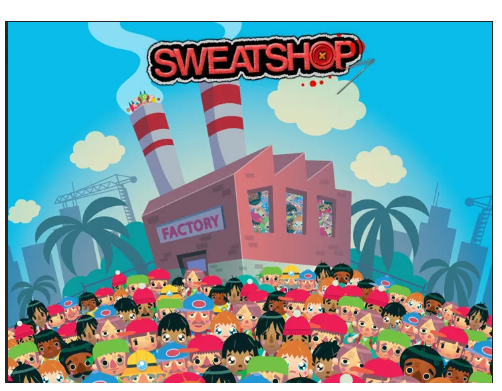
\includegraphics[width = 0.5\textwidth]{sweatshop.png}
\caption{Hra Sweatshop}
\label{fig:game}
\end{figure}
\paragraph{Spoločenské súvislosti - sociálny vplyv serióznych hier.} Seriózne hry neslúžia len na odovzdávanie informácií, ale často je za nimi ukrytý hlbší zámer, pričom účelom hry je ho naplniť. Má to byť nejaká forma osvety o téme, o ktorej si tvorcovia hry myslia, že o nej má zmyseľ hovoriť. Samozrejme, skutočným zámerom nie je len otvorenie dialógu, pretože ten má eventuálne viesť k činom a skutkom. Hra z predošlého odseku je skvelým príkladom takej hry - jej cieľom je obmedzenie vykorisťovania chudobných zamestnancov továrne manažérmi a firmou. Hoci táto továreň je fiktívna, v skutočnom svete je veľa firiem, ktoré tieto špinavé praktiky praktizujú. Iné známejšie hry s priamymi účelmi sú ICED, ktorá kritizuje nehumánne zaobchádzanie s migrantami v niektorých krajinách, alebo Fate of the World, ktorá je zameraná na klimatické zmeny.
\paragraph{Herné mechaniky, zábava, príbeh.} Toto sú vlastnosti, ktoré seriózne hry zdieľajú s komerčnými hrami a sú nevyhnutnou súčasťou ich dizajnu, keďže reprezentujú aspekt zábavy a sú výsledkom kreatívnej tvorby obsahu a programovania softvéru. Tomu, ako by sa mali optimálne implementovať sa venuje časť \ref{riesenie}.

\section{Nedostatky serióznych hier} \label{problem}
Aby bolo možné plne pochopiť tento problém, treba sa najprv pozrieť na definíciu serióznej hry a ako sa bežne odlišuje od bežnej hry. Hry komerčného typu slúžia všeobecne na zábavu a oddych a pri ich tvorbe sa toto berie ako primárny faktor, zatiaľ čo seriózny hry sa, ako sa už spomínalo, zameriavajú na akademické alebo profesijné prostredie a majú silný poučný charakter, zodpovedajúci ortodoxným koncepciám ich tvorby. Na dosiahnutie tohto cieľa využíva vedná disciplína serióznych hier teórie učenia, ktorá sa vyvíjali popri samotnom vzdelávacom systéme a akademickom prostredí, čím sa líši od komerčných hier. Herná teória, ktorá je tiež vedecky formulovaná a je extenzívne popísaná napríklad tu \cite{owen2013game} sa totiž na ne priamo neodvoláva. Teórie, ktoré tvoria podklad serióznych hier a frameworky, ktoré tieto teórie aplikujú, popisujú časti \ref{jadro:teorie} a \ref{jadro:frameworky} .

Definície serióznych hier a hier komerčných teda predpokladajú, že zamýšľaný cieľ a praktický efekt na hráča sú rozdielne. No napriek tomu, že sa takto tieto dva typy hier odlišujú, tak po hlbšom preskúmaní je jasné, že existuje silné prekrytie medzi týmito dvomi sférami. Ako príklad sa dá uviesť napríklad strategická hra z obdobia neskorého stredoveku, renesancie a baroka Europa Universalis II, ktorá podľa \cite{egenfeldt2012europa} je excelentným nástrojom, ktorým možno učiť históriu tohto obdobia. Hra síce dáva hráčovi určitú voľnosť, ako reagovať na rôzne udalosti v hre, tie sú však generované s ohľadom na skutočnú históriu, schopnosti a efektívnosť jednotlivých panovníkov zodpovedajú historickej realite atď. EUII je teda nielen klasická komerčná hra, ale dokáže v podstate aj spĺňať rolu serióznej hry. Ďalším príkladom komerčnej hry, ktorá môže byť použitá na účely serióznej hry, je (podľa zhodnotenia štúdiou \cite{backlund2013educational}) hra Tainio, ktorá je skvelá na učenie sa rôznych jazykov.
Rovnako sa dá argumentovať, že niektoré seriózne hry sú v praktickom prevedení primárne zábavné a ich poučný charakter je silno zatienený. Z toho vyplýva, že mnoho komerčných hier (prinajmenšom všetky historicky orientované strategické hry a všetky realistické simulátory, napríklad letecké simulátory) majú vzdelávací potenciál (a v niektorých prípadoch boli použité aj presne na tieto účely), zatiaľ čo mnohé seriózne hry, ktoré boli pre tento účel vytvorené, zlyhávajú. Odpoveďou na to, prečo to tak je, by mohla byť napríklad táto definícia hier (komerčných): \emph{hra je aktivita riešiaca problém, ku ktorej sa pristupuje s hravým postojom} \cite{schell2008art}. Keďže vyriešenie daného problému vyžaduje pochopenie herných mechaník a systémov a aplikovanie tohto porozumenia, je možné pripustiť, že každá aspoň trochu komplikovane štruktúrovaná hra má implicitne za cieľ nejaké porozumenie/pochopenie a hráči ho hľadajú intuitívne. A keďže mnohé komerčné hry dokážu v tomto virtuálnom prostredí za daný cieľ stanoviť porozumenie/poučenie, ktoré má využitie v reálnom svete, tak práve tu by mohlo existovať riešenie základného problému serióznych hier - poskytnúť hráčovi dostatok zábavy a zároveň šikovne pripojiť edukatívne prvky do nich tak, aby ich chcel intuitívne zvládnuť, čím sa vytvorí motivácia a, ideálne, aj dlhodobý efekt na hráča. Toto poznanie sa dá implikačne vyvodiť aj z teórií, ktoré slúžia na vývoj serióznych hier \ref{jadro:teorie}.

\section{Teórie učenia a koncepcie herného vývoja} \label{jadro}
Hoci pedagogické teórie zamerané na seriózne hry sú relatívne nové, čerpajú z bohatej histórie teórií a predstáv o učení a o tom, ako efektívne učiť a vzdelávať, keďže filozofia sa s týmto problémom zapodievala už od čias Platóna a Aristotela. Mnohí veľkí myslitelia si totiž uvedomovali, že ovplyvnením mladej generácie ich doby môžu nepriamo vplývať na ďalší chod a progres spoločnosti. V posledných stáročiach sa vyvinuli rôzne metodiky učenia, z ktorých, ako uvádza \cite{natucci2021experience}, sa vyvinuli teórie učenia spojené so serióznymi hrami.

\subsection{Teórie učenia} \label{jadro:teorie}
4 prístupy a chápania učenia relevantné pri vývoji serióznych hier:

1. Konštruktivizmus - predpokladá, že subjekt, ktorý sa učí, je aktívny konštruktor informácií, teda učenie je priamo naviazané na predošlé poznatky a novoprijaté informácie sa posudzujú podľa predošle získaných vedomostí

2. Sociokonštruktivizmus - variant konštruktivizmu, konštruktorom informácií sú sociálne štruktúry a interakcie, ktoré priamo ovplyvňujú subjekt učenia

3. Kognitivizmus - nevyhnutnou súčasťou procesu učenia je premýšľanie a implikuje, že najefektívnejší spôsob pochopenia a uloženia informácie do pamäte je štrukturalizácia obsahu učenia od jednoduchému ku komplexnému (uprednostňuje teda analytický prístup)

4. Humanizmus - predpokladá, že učenie je individuálne v zmysle, že okrem kognitívnych parametrov treba brať do úvahy osobné potreby a hodnoty jednotlivca - subjektu

Tieto základné prístupy a ich prípadné modifikácie slúžia na modelovanie frameworkov serióznych hier \ref{jadro:frameworky} - nesúvisia len so samotným učením, ale ovplyvňujú aj to, ako sú chápané koncepty ako je zábava, relax, atď. Ich spojením je celkom jasné, že človek si novozískané informácie omnoho ľahšie osvojí v prípade, že sú mu podané cestou, ktorá mu nepríde ako vnútená - inými slovami, najlepšie si človek zapamätá to, čo si zapamätať chce a práve preto je v serióznych hrách tak dôležité nebrať ohľad len na "seriózne", ale aj na "hry".

\subsection{Súčasné koncepcie herného vývoja - frameworky} \label{jadro:frameworky}
Podľa zdroja \cite{natucci2021experience} sú toto najpopulárnejšie frameworky vývoja serióznych hier:

1. \emph{The Mechanics, Dynamics, and Aesthetics Framework} (MDA) - skladá sa z 3 základných komponentov - mechaniky, ktoré reprezentujú dáta a algoritmy, z ktorých hra pozostáva; dynamiky, ktoré popisujú správanie hry a interakciu s ľudským hráčom; estetiky, ktoré požadujú očakávané emočné a mentálne reakcie na obsah hry. Tento framework prikladá veľkú váhu zábave a výučba je skôr druhoradá.

2. \emph{The Elemental Tetrad - The Aesthetics, Mechanics, Technology, and Story Framework} (AMTS) - estetiky - v tomto prípade definované ako blueprint vzhľadu a pocitu z hry; mechaniky ako cieľ hry; technológie ako hardvér a výrobný materiál, príbeh ako hlavný generátor udalostí v hre. Práve na príbeh sa kladie najväčší dôraz.

3. \emph{The Design, Play and Experience Framework} (DPE) je nadstavba MDA, ktorá však berie veľký ohľad aj na vzdelávací aspekt a rozdelenie priorít expanduje na 5 kategórií - vzdelávanie (edukatívne elementy), príbeh, hrateľnosť (podobné ako mechaniky v MDA), perspektíva používateľa (nadväzuje na dynamiky MDA) a technológie, ktoré predstavujú technické limitácie vývojárskeho tímu. Tento framework je všeobecne považovaný za najlepší v oblasti vyváženosti, no má svoje nedostatky. Jeho tvorcovia napríklad pri dizajne tohto frameworku netestovali dlhodobú efektivitu týchto hier, ani nebrali príliš ohľad na veci, ktoré dotvárajú atmosféru hry (hudobný sprievod, pokročilé pohyby, hladké 3D animácie,...)

Tu \ref{fig:table} môžeme vidieť zoznam 10 najvplyvnejších serióznych hier, pričom všetky využívajú niektorý z týchto frameworkov:
\begin{figure}[h]
\centering
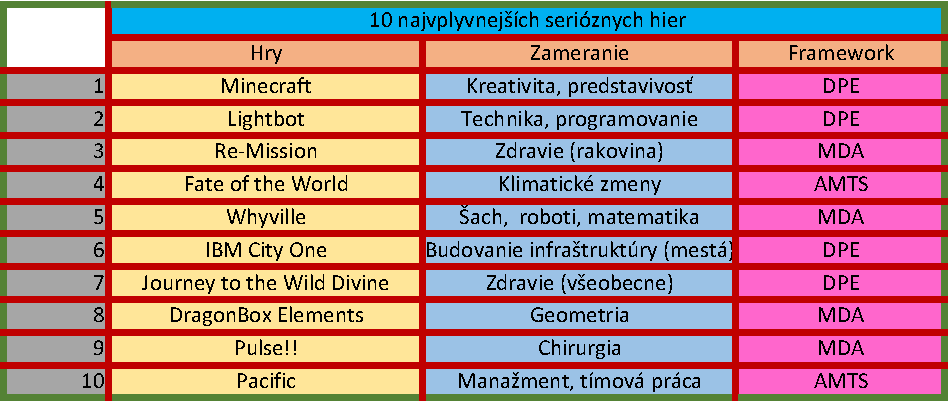
\includegraphics[width = 0.8\textwidth]{uspesne_ser_hry.pdf}
\caption{Najvplyvnejšie hry podľa \url{https://www.linkedin.com/pulse/top-10-serious-games-all-time-juliette-denny}}
\label{fig:table}
\end{figure}

\section{Predostretie optimálnej koncepcie a štruktúry vývoja} \label{riesenie}
Z predošlých analýz a úvah ako aj tejto, tak aj rozličných publikovaných prác (mnohé z uvedených zdrojov sa tomuto venujú) je očividné, že aj framework optimalizovaný pre riešenia nedostatkov serióznych hier sa snaží dosiahnuť určitý, jasne vyhranený cieľ, ktorý presahuje hru samotnú. Ak by to nezvládla, zmysel jej existencie by nebol dosiahnutý. Hra preto musí byť štruktúrovaná okolo tohto cieľa, no musí byť aj koherentná a zároveň musí adekvátne implementovať zábavné a relaxačné prvky.

Tu však nastáva jeden problém. Vo sfére psychológie je dlhodobo známy fakt, že ľudia sú rozliční a veľmi individuálni. V tomto kontexte je jasné, že seriózna hra, akokoľvek dobre namodelovaná, nedokáže zaručiť prenos požadovaných informácií na každého hráča, rozhodne nie s rovnakým účinkom. Očakávať opak je nerealistické. Možno sa spoliehať len na to, že \emph{štruktúra hry ovplyvňuje priestor možností (preniesť vedomosť) samotnej hry} \cite{mitgutsch2012purposeful}.

Popri tomto všetkom však treba myslieť aj na klasické prvky hier - herné mechaniky, grafický, postavy (pravdepodobne hra má hlavnú postavu ovládanú hráčom a vedľajšie postavy ovládané umelou inteligenciou), naratív, celková atmosféra, funkčnosť. Treba ich konštruovať tak, aby vyvolali v hráčovi pocit silnej imerzie do hry, pretože v takom prípade má hra silný dopad na podvedomie človeka a dokáže ho ovplyvňovať \cite{an2015subconscious}. Najsilnejšími aktérmi v tomto ohľade sú práve zvuk a obraz. Je všeobecne známe, že zvukový sprievod (angl. soundtrack sa používa častejšie) je veľmi dôležitou súčasťou každej hry - mnohé z populárnych (komerčných) hier vynikajú svojím soundtrackom a aj mnohé hry vyvíjané nezávislými tímami (tzv. indie hry) majú unikátne soundtracky. Je však vzácne, aby seriózna hra dbala vo väčšej miere o tento aspekt hry. Čo sa týka obrazu, už som spomenul, že tvorcovia veľmi nedbajú na pokročilé vizuálne prvky. Je to pochopiteľné, keďže dôležitejšie je poslanie hry a čo dokáže naučiť, no keďže hráči očakávajú štandardne nejakú kvalitu animácií, ktoré vyzerajú dobre, ale zároveň nespomaľujú beh hry a nespôsobujú sekanie či dlhé načítavanie, veľmi by to pomohlo s predajom hry, čo by samozrejme spôsobilo aj šírenie jej vzdelávacieho poslania. Samozrejme, v jadre každej dobrej hry je aj nejaký príbeh, ktorý hru posúva a posilňuje jej záživnosť a napínavosť.

V skratke, seriózne hry by skutočne boli úspešnejšie, ak by sa viac inšpirovali komerčne úspešnými hrami. Príkladom toho sú aj tieto hry \ref{fig:table}, z ktorých sú mnohé, najmä Minecraft, často vnímané ako komerčné hry.

\section{Zhrnutie} \label{zaver}
Metodologickým postupom (uvedenie témy, pochopenie témy a problému, analýza vedeckých faktov z relevantných oblastí, riešenie problému použitím vedeckých štúdií a mojich úvah) som prišiel k týmto záverom: Seriózne hry sú novodobým nástrojom výuky o dôležitých témach, ktorý má veľký potenciál sa uplatňovať v akademickej oblasti na globálnej úrovni. Hlavným problémom týchto programov býva, že sa príliš snažia vzdelávať bez akýchkoľvek stimulantov, ktoré by podporovali ľudský mozog v prijímaní a aplikovaní týchto informácií. Príklady niektorých komerčných hier, ktoré majú veľkú vzdelávaciu hodnotu, ukázali, že modelovanie budúcich serióznych hier by sa malo nimi inšpirovať a viacej implementovať niektoré záživné a zábavné prvky komerčných hier. Toto jednoznačne zlepší krátkodobé i dlhodobé ukladanie týchto informácií a skôr povedie k ich aplikácii, čoho príkladom sú tie najvplyvnejšie seriózne hry, ktoré všeobecne brali väčší ohľad na tieto veci. Preto by sa na tvorbu serióznych hier mal vytvoriť framework, ktorý bude stavať na tom, v čom sú už existujúce frameworky dobré ale bude brať ohľad aj na tieto veci.

\bibliographystyle{plain}
\bibliography{zdroje}

\end{document}









